%!TEX program = lualatex
\documentclass[11pt,class=beamer]{standalone}
\usepackage{etoolbox}
\usepackage{ifxetex}
\usepackage{ifluatex}
\usepackage[T1]{fontenc}
\ifboolexpr{bool{xetex} or bool{luatex}}{%
	\usepackage{fontspec}
}{%
	\usepackage[utf8]{inputenc}
}
\usepackage{xcolor}

\usepackage{amsmath}
\usepackage{amssymb}
\usepackage{mathrsfs}
\usepackage{braket}

\usepackage{pgf}
\usepackage{tikz}
\usepackage{tikzpeople}

\usepackage{array}
\usepackage{tabularx}
\usepackage{multirow}

\usetikzlibrary{shapes}
\usetikzlibrary{arrows.meta}
\usetikzlibrary{calc}
\usetikzlibrary{positioning}
\usetikzlibrary{angles}
\usetikzlibrary{quotes}
\usetikzlibrary{decorations}

\definecolor{bg_color}{RGB}{250,250,229}
\definecolor{Cblue}{RGB}{38,75,150}
\definecolor{Cgreen}{RGB}{39,179,118}
\definecolor{Cdarkgreen}{RGB}{0,111,60}
\definecolor{Corange}{RGB}{249,167,62}
\definecolor{Cred}{RGB}{191,33,47}

\colorlet{good}{green!90!black}
\colorlet{average}{Corange}
\colorlet{bad}{Cred}


\beamertemplatenavigationsymbolsempty{}

\begin{document}
	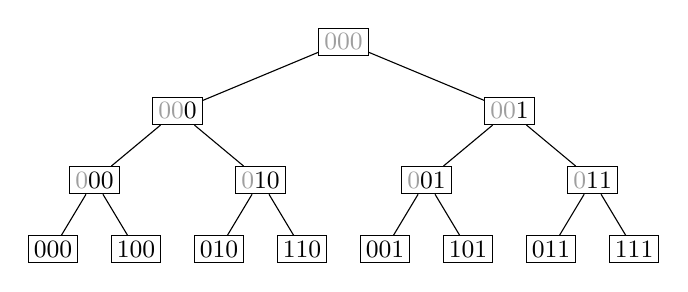
\begin{tikzpicture}[
		x=1pt,
		y=1pt,
		/utils/exec={\sffamily},
		font=\fontsize{9pt}{9.5pt}\selectfont,
		>=Triangle,
		decoration={snake,segment length=5,amplitude=0.7},
		level distance=25,
		level 1/.style={sibling distance=120},
		level 2/.style={sibling distance=60},
		level 3/.style={sibling distance=30}
	]
		\tikzset{bitset/.style={
			draw,
			rectangle,
			inner sep=2,
		}}

		\node[bitset] {\(\color{gray!75}000\)}
			child {
				node[bitset] {\({\color{gray!75}00}0\)}
				child {
					node[bitset] {\({\color{gray!75}0}00\)}
					child {
						node[bitset] {\(000\)}
					}
					child {
						node[bitset] {\(100\)}
					}
				}
				child {
					node[bitset] {\({\color{gray!75}0}10\)}
					child {
						node[bitset] {\(010\)}
					}
					child {
						node[bitset] {\(110\)}
					}
				}
			}
			child {
				node[bitset] {\({\color{gray!75}00}1\)}
				child {
					node[bitset] {\({\color{gray!75}0}01\)}
					child {
						node[bitset] {\(001\)}
					}
					child {
						node[bitset] {\(101\)}
					}
				}
				child {
					node[bitset] {\({\color{gray!75}0}11\)}
					child {
						node[bitset] {\(011\)}
					}
					child {
						node[bitset] {\(111\)}
					}
				}
			};
	\end{tikzpicture}
\end{document}%